\documentclass[a4paper, 14pt]{article}
\usepackage{tocloft}

\usepackage{amsthm}
\newtheorem{theorem}{Теорема}
\newtheorem{lemma}{Лемма}

\usepackage{setspace}
%\полуторный интервал
\onehalfspacing

\usepackage{arxiv}

\usepackage[T2A]{fontenc}
\usepackage[utf8]{inputenc}
\usepackage[english, russian]{babel}
% \usepackage{cmap}
\usepackage{url}
\usepackage{booktabs}
\usepackage{nicefrac}
\usepackage{microtype}
\usepackage{lipsum}
\usepackage{graphicx}
\usepackage{subfig}
\usepackage[square,sort,comma,numbers]{natbib}
\usepackage{doi}
\usepackage{multicol}
\usepackage{multirow}
\usepackage{tabularx}
\usepackage{color,colortbl} % Раскраска таблицы
\definecolor{Gray}{gray}{0.9}

\usepackage{tikz}
\usetikzlibrary{matrix}

% Algorithms
\usepackage{algpseudocode}
\usepackage{algorithm}

%% Шрифты
\usepackage{euscript} % Шрифт Евклид
\usepackage{mathrsfs} % Красивый матшрифт
\usepackage{extsizes} % Возможность сделать 14-й шрифт

\usepackage{makecell} % diaghead in a table
\usepackage{amsmath,amsfonts,amssymb,amsthm,mathtools,dsfont}
\usepackage{icomma}

\newcommand{\bz}{\mathbf{z}}
\newcommand{\bx}{\mathbf{x}}
\newcommand{\by}{\mathbf{y}}
\newcommand{\bv}{\mathbf{v}}
\newcommand{\bw}{\mathbf{w}}
\newcommand{\ba}{\mathbf{a}}
\newcommand{\bb}{\mathbf{b}}
\newcommand{\bp}{\mathbf{p}}
\newcommand{\bq}{\mathbf{q}}
\newcommand{\bt}{\mathbf{t}}
\newcommand{\bu}{\mathbf{u}}
\newcommand{\bs}{\mathbf{s}}
\newcommand{\bT}{\mathbf{T}}
\newcommand{\bX}{\mathbf{X}}
\newcommand{\bZ}{\mathbf{Z}}
\newcommand{\bS}{\mathbf{S}}
\newcommand{\bH}{\mathbf{H}}
\newcommand{\bW}{\mathbf{W}}
\newcommand{\bY}{\mathbf{Y}}
\newcommand{\bU}{\mathbf{U}}
\newcommand{\bQ}{\mathbf{Q}}
\newcommand{\bP}{\mathbf{P}}
\newcommand{\bA}{\mathbf{A}}
\newcommand{\bB}{\mathbf{B}}
\newcommand{\bC}{\mathbf{C}}
\newcommand{\bE}{\mathbf{E}}
\newcommand{\bF}{\mathbf{F}}
\newcommand{\bomega}{\boldsymbol{\omega}}
\newcommand{\btheta}{\boldsymbol{\theta}}
\newcommand{\bgamma}{\boldsymbol{\gamma}}
\newcommand{\bdelta}{\boldsymbol{\delta}}
\newcommand{\bPsi}{\boldsymbol{\Psi}}
\newcommand{\bpsi}{\boldsymbol{\psi}}
\newcommand{\bxi}{\boldsymbol{\xi}}
\newcommand{\bchi}{\boldsymbol{\chi}}
\newcommand{\bzeta}{\boldsymbol{\zeta}}
\newcommand{\blambda}{\boldsymbol{\lambda}}
\newcommand{\beps}{\boldsymbol{\varepsilon}}
\newcommand{\bZeta}{\boldsymbol{Z}}
% mathcal
\newcommand{\cX}{\mathcal{X}}
\newcommand{\cY}{\mathcal{Y}}
\newcommand{\cW}{\mathcal{W}}

\newcommand{\dH}{\mathds{H}}
\newcommand{\dR}{\mathds{R}}
% transpose
\newcommand{\T}{^{\mathsf{T}}}

% \renewcommand{\shorttitle}{\textit{arXiv} Шаблон}
\renewcommand{\epsilon}{\ensuremath{\varepsilon}}
\renewcommand{\phi}{\ensuremath{\varphi}}
\renewcommand{\kappa}{\ensuremath{\varkappa}}
\renewcommand{\le}{\ensuremath{\leqslant}}
\renewcommand{\leq}{\ensuremath{\leqslant}}
\renewcommand{\ge}{\ensuremath{\geqslant}}
\renewcommand{\geq}{\ensuremath{\geqslant}}
\renewcommand{\emptyset}{\varnothing}

\usepackage{hyperref}
% \usepackage[usenames,dvipsnames,svgnames,table,rgb]{xcolor}

\hypersetup{
	unicode=true,
	pdftitle={A template for the arxiv style},
	pdfsubject={q-bio.NC, q-bio.QM},
	pdfauthor={David S.~Hippocampus, Elias D.~Striatum},
	pdfkeywords={First keyword, Second keyword, More},
	colorlinks=true,
	linkcolor=black,        % внутренние ссылки
	citecolor=blue,         % на библиографию
	filecolor=magenta,      % на файлы
	urlcolor=blue           % на URL
}

\graphicspath{{../figures/}}

\usepackage{enumitem} % Для модификаций перечневых окружений

\theoremstyle{definition} % "Определение"
\newtheorem{definition}{Опр.}[section]

\usepackage{etoolbox}

\makeatletter
\expandafter\patchcmd\csname\string\algorithmic\endcsname{\itemsep\z@}{\itemsep=1.5mm}{}{}
\makeatother
%%% Титульный лист
% \input{title}
% \setcounter{page}{2}

\renewcommand{\abstractname}{Аннотация}

\title{Методы векторного представления глубоких генеративных моделей}

\author{
    Мария Никитина \\
    \texttt{nikitina.mariia@phystech.edu} \\
    \And
    Антон Бишук \\
    \texttt{anton.bishuk@mail.ru} \\
    \And
    Олег Бахтеев \\
    \texttt{bakhteev(at)phystech.edu}
}
\date{\today}

\usepackage{setspace}
%\полуторный интервал
\onehalfspacing

\begin{document}
\maketitle
% \input{title}
\setcounter{page}{2}

\begin{abstract}
Увеличение времени и ресурсов, затрачиваемых на обучение больших моделей привели к появлению большого количества работ, направленных на поиск уже существующей обученной модели, подходящей под новую задачу. Множество исследований направлено на поиск пространства моделей-датасетов, с помощью которого можно отыскать уже существующую модель, хорошо подходящую под новую задачу. Однако, исследования проводятся в основном в области дискриминативных моделей. Эта работа направлена на поиск векторного представления генеративных моделей, описывающего статистические свойства датасетов, на которых они обучены. Таким образом с помощью такого пространства можно подбирать подходящую генеративную модель, используя привычные операции с векторами. Эксперименты проводятся на VAE и Autoencoder.
\end{abstract}

% \keywords{Генеративные модели \and Векторное представление \and Статистические свойства моделей}

\newpage
% \pagenumbering{roman} % use lowercase Roman numerals for page numbering before the main content

% \tableofcontents
% \clearpage % start the table of contents on a new page

% \pagenumbering{arabic}

\section{Введение}
Пусть задан некоторый набор генеративных моделей, описывающий разные выборки/генеральные совокупности данных. Требуется предложить метод векторного представления этих моделей, который будет сохранять статистические свойства данных. С помощью такого представления можно облегчить поиск подходящей обученной модели  без больших затрат времени и ресурсов на обучения. Также поиск по пространству генеративных моделей может быть применим для анализа качества работы разных архитектур на задаче генерации требуемых данных.

Векторное пространство должно отвечать следующим требованиям:

\begin{enumerate}
    \item Расстояние между векторными представлениями моделей для близких выборок должно быть невелико (при условии, что сами модели хорошо их описывают);

    \item Модели, обученные на композиции/смеси выборок должны учитывать свойства всех выборок, входящих в смесь.
\end{enumerate}

Для выполнения данных требования и решения задачи в данной статье исследуются и сравниваются три варианта решения:

\begin{enumerate}
    \item Один из возможных вариантов: сумма векторных представлений моделей, полученных по датасетам $D_1$, $D_2$ должна приблизительно соответствовать векторному представлению датасета $D_1 + D_2$. Пример для итогового пространства в виде единичной сферы представлен на рис. \ref{fg:classes};
    
    \item Вместо использования евклидового расстояния на векторных представлениях, использовать иерархию;
    
    \item Представить модель как граф и работать с пространством графов.
\end{enumerate}

\begin{figure}
    \begin{center}
    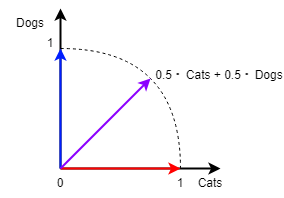
\includegraphics[width=0.7\linewidth]{Presentation/Pictures/Classes.png}
    \caption{Требуемое соотношение между моделями в векторном пространстве}
    \label{fg:classes}
    \end{center}
\end{figure}

\section{Связанные работы}
Существует большое количество работ, направленных на использование энкодера поверх других моделей. Но большинство из них используют дискриминативные модели. Например, энкодер и диффузия \citep{Encoder_diffusion}, кодирование модели NAS \citep{NAS} или целый набор векторов из раздичных моделей \citep{TANS}.

Изучение представлений помогает понять закономерности в работе нейронных сетей. В \citep{SANE} представлен метод SANE. Он обучает универсальные представления нейронных сетей, которые масштабируются для больших моделей различных архитектур и предназначенных для разных задач. Для решения SANE испрользует гиперпредставления для последовательной обработки подмножеств весов нейронной сети, что позволяет представить большие нейронные сети как набор токенов и перевести в пространство представления.

В данной работе большое внимание будет уделено кодированию модели с помощью сингулярных чисел её весов. Описание свойств сингулярных чисел в модели представлено в \citep{Singular}.

\section{Вазимная информация модели и данных}

Чтобы оценить возможность модели описывать данные, на которых она обучалась, необходимо оценить потери информации между исходными данными, весами модели при обучении подвыбоке и последующей векторизацией. Для оценки используется такая метрика, как совместная информация:

\[I(X; Y) = HY - H(Y \mid X).\]

\begin{theorem}
\label{thm:info}
$X = \{\mathbf{x}_1, \dots, \mathbf{x}_n\} \in \mathbb{R}^{n \times d}$ -- множество независимых векторов (пусть $\mathbf{x}_i \in \mathbb{R}^d$ и $\mathbf{x}_i \sim \mathcal{N}(\boldsymbol{\mu}, \boldsymbol{\Sigma})$).

$X_1 \in \mathbb{R}^{m \times d}$ -- его подмножество, формируемое путём независимого включения каждого вектора $\mathbf{x}_i$ с вероятностью $p$.

$AE$ -- линейный автоэнкодер с весами $W \in \mathbb{R}^{k\times d}$. $AE$ обучен на $X_1$, то есть $W = W(X_1)$.

Тогда имеем следующие попарные взаимные информации:

\begin{enumerate}
    \item \[I(X; X_1) \approx np \cdot H(\mathbf{x}_i), ~~~  H(\mathbf{x}_i) = \frac{1}{2} \log \left( (2 \pi e)^d |\Sigma| \right);\]

    \item \[I(X_1; \mathbf{W}) = \frac{m}{2} \log \frac{|\boldsymbol{\Sigma}|}{|(\mathbf{I} - \mathbf{W}_2 \mathbf{W}_1) \boldsymbol{\Sigma} (\mathbf{I} - \mathbf{W}_2 \mathbf{W}_1)^T|}\]

    \item \[I(X_1; \mathbf{S}) \approx \frac{m}{4} \log \left( (2\pi e)^k \prod_{i=1}^k \lambda_i^2 \right).\]
\end{enumerate}
\end{theorem}

\begin{proof}
\begin{enumerate}
    \item Обозначим индикаторы включения $Z_i \sim \text{Bernoulli}(p)$, тогда $X_1 = \{ \mathbf{x}_i \mid Z_i = 1 \}$.

Поскольку $X_1$ однозначно определяется $X$ и $Z = (Z_1, \dots, Z_n)$, то:
\[H(X_1 \mid X) = H(Z \mid X) = H(Z),\]

так как $Z$ не зависит от $X$ (выбор подмножества случайный и независимый от значений векторов).

Таким образом:
\[I(X; X_1) = H(X_1) - H(Z).\]

Так как $Z_i$ независимы и $Z_i \sim \text{Bernoulli}(p)$, то:
\[H(Z) = \sum_{i=1}^n H(Z_i) = n H_{\text{bin}}(p),\]

\noindent где $H_{\text{bin}}(p) = -p \log p - (1-p) \log (1-p)$ -- энтропия Бернулли.

Подмножество $X_1$ состоит из случайного числа $m = \sum_{i=1}^n Z_i$ векторов (где $m \sim \text{Binomial}(n, p)$), и для каждого фиксированного $m$ векторы в $X_1$ — это $m$ независимых векторов.  

Таким образом, условная энтропия при фиксированном $m$:
\[H(X_1 \mid m) = m \cdot H(\mathbf{x}_i) = m \cdot \frac{1}{2} \log \left( (2 \pi e)^d |\Sigma| \right).\]

Тогда полная энтропия:
\[H(X_1) = \sum_{m=0}^n P(m) \cdot H(X_1 \mid m) + H(m),\]

\noindent где $H(m)$ — это энтропия биномиального распределения:
\[H(m) = H_{\text{binomial}}(n, p).\]

Тогда:
\[H(X_1) = H(m) + \mathbb{E}[H(X_1 \mid m)] = H_{\text{binomial}}(n, p) + \mathbb{E}[m] \cdot H(\mathbf{x}_i).\]

Поскольку $\mathbb{E}[m] = np$, то:
\[H(X_1) = H_{\text{binomial}}(n, p) + np \cdot \frac{1}{2} \log \left( (2\pi e)^d |\Sigma| \right).\]

Для взаимной информации получаем:
\[I(X; X_1) = H_{\text{binomial}}(n, p) + n p \cdot \frac{1}{2} \log \left( (2 \pi e)^d |\Sigma| \right) - n H_{\text{bin}}(p).\]

При $n \to \infty$: $H_{\text{binomial}}(n, p) \approx n H_{\text{bin}}(p)$. Тогда:
\[I(X; X_1) \approx np \cdot \frac{1}{2} \log \left( (2 \pi e)^d |\Sigma| \right).\]

    \item Автоэнкодер (линейный, без активаций):

Кодировщик: $\mathbf{z} = \mathbf{W}_1 \mathbf{x} + \mathbf{b}_1$

Декодировщик: $\mathbf{\hat{x}} = \mathbf{W}_2 \mathbf{z} + \mathbf{b}_2$

Выход автоэнкодера: 
\[\mathbf{\hat{x}} = \mathbf{W}_2 \mathbf{W}_1 \mathbf{x} + \mathbf{W}_2\mathbf{b}_1 + \mathbf{b}_2\]  

Обозначим $\mathbf{A} = \mathbf{W}_2 \mathbf{W}_1$, $\mathbf{c} = \mathbf{W}_2 \mathbf{b}_1 + \mathbf{b}_2$. Тогда:
\[\mathbf{\hat{x}} = \mathbf{A} \mathbf{x} + \mathbf{c}\]  

Поскольку $\mathbf{x}$ гауссовский, а $\mathbf{\hat{x}}$ — его линейное преобразование, то:
\[\mathbf{\hat{x}} \sim \mathcal{N}(\mathbf{A} \boldsymbol{\mu}_x + \mathbf{c}, \mathbf{A} \boldsymbol{\Sigma} \mathbf{A}^T)\]  

Ошибка восстановления:  
\[\boldsymbol{\epsilon} = \mathbf{x} - \mathbf{\hat{x}} = (\mathbf{I} - \mathbf{A}) \mathbf{x} - \mathbf{c}\]  

\[\boldsymbol{\epsilon} \sim \mathcal{N}\left( (\mathbf{I} - \mathbf{A}) \boldsymbol{\mu}_x - \mathbf{c}, (\mathbf{I} - \mathbf{A}) \boldsymbol{\Sigma} (\mathbf{I} - \mathbf{A})^T \right)\]  

Взаимная информация между $\mathbf{x}$ и весами $\mathbf{W} = (\mathbf{W}_1, \mathbf{W}_2)$:
\[I(\mathbf{x}; \mathbf{W}) = H(\mathbf{x}) - H(\mathbf{x} | \mathbf{W})\]  

Для гауссовского вектора:  
\[H(\mathbf{x}) = \frac{1}{2} \log \left( (2\pi e)^d |\boldsymbol{\Sigma}| \right)\]  

Условное распределение $\mathbf{x}$ при фиксированных $\mathbf{W}$ определяется ошибкой $\boldsymbol{\epsilon}$:  
\[H(\mathbf{x} | \mathbf{W}) = H(\boldsymbol{\epsilon}) = \frac{1}{2} \log \left( (2\pi e)^d |(\mathbf{I} - \mathbf{A}) \boldsymbol{\Sigma} (\mathbf{I} - \mathbf{A})^T| \right)\]  

Подставляем $H(\mathbf{x})$ и $H(\mathbf{x}|\mathbf{W})$:  
\[I(\mathbf{x}; \mathbf{W}) = \frac{1}{2} \log \frac{|\boldsymbol{\Sigma}|}{|(\mathbf{I} - \mathbf{A}) \boldsymbol{\Sigma} (\mathbf{I} - \mathbf{A})^T|}\]  
\noindent где $\mathbf{A} = \mathbf{W}_2 \mathbf{W}_1$.  

Если автоэнкодер обучен как PCA (т.е. $\mathbf{W}_1 = \mathbf{U}^T$, $\mathbf{W}_2 = \mathbf{U}$, где $\mathbf{U}$ — матрица главных компонент), то:  
\[\mathbf{A} = \mathbf{U} \mathbf{U}^T\]  

Ковариация ошибки:  
\[(\mathbf{I} - \mathbf{U} \mathbf{U}^T) \boldsymbol{\Sigma} (\mathbf{I} - \mathbf{U} \mathbf{U}^T)^T = \boldsymbol{\Sigma} - \mathbf{U} \mathbf{\Lambda} \mathbf{U}^T\]  
где $\mathbf{\Lambda}$ — диагональная матрица собственных значений.  

Тогда:  
\[I(\mathbf{x}; \mathbf{W}) = \frac{1}{2} \log \frac{|\boldsymbol{\Sigma}|}{|\boldsymbol{\Sigma} - \mathbf{U} \mathbf{\Lambda} \mathbf{U}^T|}\]  

Если $\mathbf{A} \approx \mathbf{I}$ (идеальное восстановление), то $|\mathbf{I} - \mathbf{A}| \approx 0$ и $I(\mathbf{x}; \mathbf{W}) \to \infty$.  

Если $\mathbf{A} \approx 0$ (автоэнкодер ничего не учит), то $I(\mathbf{x}; \mathbf{W}) \approx 0$. 

Для линейного автоэнкодера и гауссовских данных взаимная информация (насколько веса модели $\mathbf{W}$ уменьшают неопределённость в данных $\mathbf{x}$) вычисляется как:  
\[I(\mathbf{x}; \mathbf{W}) = \frac{1}{2} \log \frac{|\boldsymbol{\Sigma}|}{|(\mathbf{I} - \mathbf{W}_2 \mathbf{W}_1) \boldsymbol{\Sigma} (\mathbf{I} - \mathbf{W}_2 \mathbf{W}_1)^T|}\]

    \item Рассмотрим линейный автоэнкодер с гауссовскими входными данными $\mathbf{x} \sim \mathcal{N}(\boldsymbol{\mu}, \boldsymbol{\Sigma})$. Пусть веса кодировщика $\mathbf{W}_1 \in \mathbb{R}^{k \times d}$ и декодировщика $\mathbf{W}_2 \in \mathbb{R}^{d \times k}$ имеют сингулярные разложения:

\[\mathbf{W}_1 = \mathbf{U}_1 \mathbf{S}_1 \mathbf{V}_1^T, \quad \mathbf{W}_2 = \mathbf{U}_2 \mathbf{S}_2 \mathbf{V}_2^T,\]

\noindentгде $\mathbf{S}_1$ и $\mathbf{S}_2$ — диагональные матрицы сингулярных чисел.

Сингулярные числа $\mathbf{s} = \{s_i\}$ весов $\mathbf{W} = (\mathbf{W}_1, \mathbf{W}_2)$ зависят от ковариации входных данных $\boldsymbol{\Sigma}$, так как обучение автоэнкодера минимизирует:

\[\mathbb{E} \|\mathbf{x} - \mathbf{W}_2 \mathbf{W}_1 \mathbf{x}\|^2.\]

В оптимальном случае (аналог PCA), $\mathbf{W}_2 \mathbf{W}_1$ соответствует проекции на главные компоненты $\mathbf{x}$, а сингулярные числа связаны с собственными значениями $\boldsymbol{\Sigma}_x$.

Взаимная информация между $\mathbf{x}$ и сингулярными числами $\mathbf{s}$:

\[I(\mathbf{x}; \mathbf{s}) = H(\mathbf{s}) - H(\mathbf{s} | \mathbf{x}).\]

Для PCA-like автоэнкодера, $\mathbf{s}$ — это корни собственных значений $\boldsymbol{\Sigma}$. Если $\boldsymbol{\Sigma}_x$ имеет спектр $\{\lambda_i\}$, то $s_i \approx \sqrt{\lambda_i}$. Тогда энтропия:

\[H(\mathbf{s}) = \frac{1}{2} \log \left( (2\pi e)^k \prod_{i=1}^k \text{Var}(s_i) \right).\]

При фиксированных $\mathbf{x}$, сингулярные числа $\mathbf{s}$ детерминированы (так как $\mathbf{W}$ обучаются на данных). Поэтому $H(\mathbf{s} | \mathbf{x}) = 0$.

Таким образом:

\[I(\mathbf{x}; \mathbf{s}) = H(\mathbf{s}) = \frac{1}{2} \log \left( (2\pi e)^k \prod_{i=1}^k \text{Var}(s_i) \right).\]

Если автоэнкодер близок к PCA, то $s_i \approx \sqrt{\lambda_i}$, где $\lambda_i$ -- собственные значения $\boldsymbol{\Sigma}$. Тогда:

\[I(\mathbf{x}; \mathbf{s}) \approx \frac{1}{4} \log \left( (2\pi e)^k \prod_{i=1}^k \lambda_i^2 \right).\]

Чем больше дисперсия сингулярных чисел $\mathbf{s}$, тем выше $I(\mathbf{x}; \mathbf{s})$.

Если $\mathbf{s}$ не зависят от $\mathbf{x}$ (например, случайные веса), то $I(\mathbf{x}; \mathbf{s}) = 0$.
\end{enumerate}
\end{proof}

\section{Вычислительные эксперименты}
\subsection{Бинарная классификация}

Если нужно создать вектор модели с требуемым свойством, то сначала следует проверить, насколько хорошо вектор модели описывает данные, используемые для обучения. Самый простой вариант: обучить $N$ автоэнкодеров на семплах из двух классов датасета, перевести их в векторы и затем построить энкодер, определяющий, на данных из какого класса была обучена модель (архитектура представлена на рис. \ref{fg:model_1}).

Чтобы не допустить переобучения классификатора и не завязываться на размерности, энкодеры векторизуются:

\begin{enumerate}
    \item Сингулярные числа весов
    \item Гистограмма значений весов (рис. \ref{fg:vectors})
\end{enumerate}

\begin{center}
\begin{figure}[!ht]
    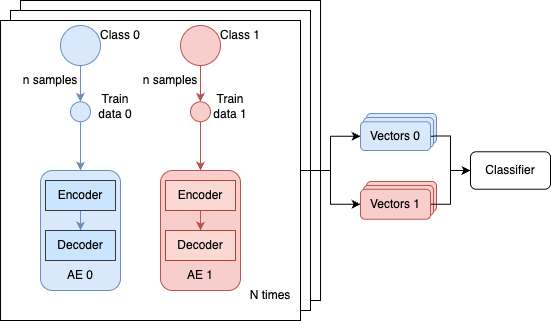
\includegraphics[width=1.0\linewidth]{Presentation/Pictures/vector_space.png}
    \caption{Архитектура эксперимента с бинарной классификацией}
    \label{fg:model_1}
\end{figure}
\end{center}

\begin{figure}[!ht]
    \begin{center}
    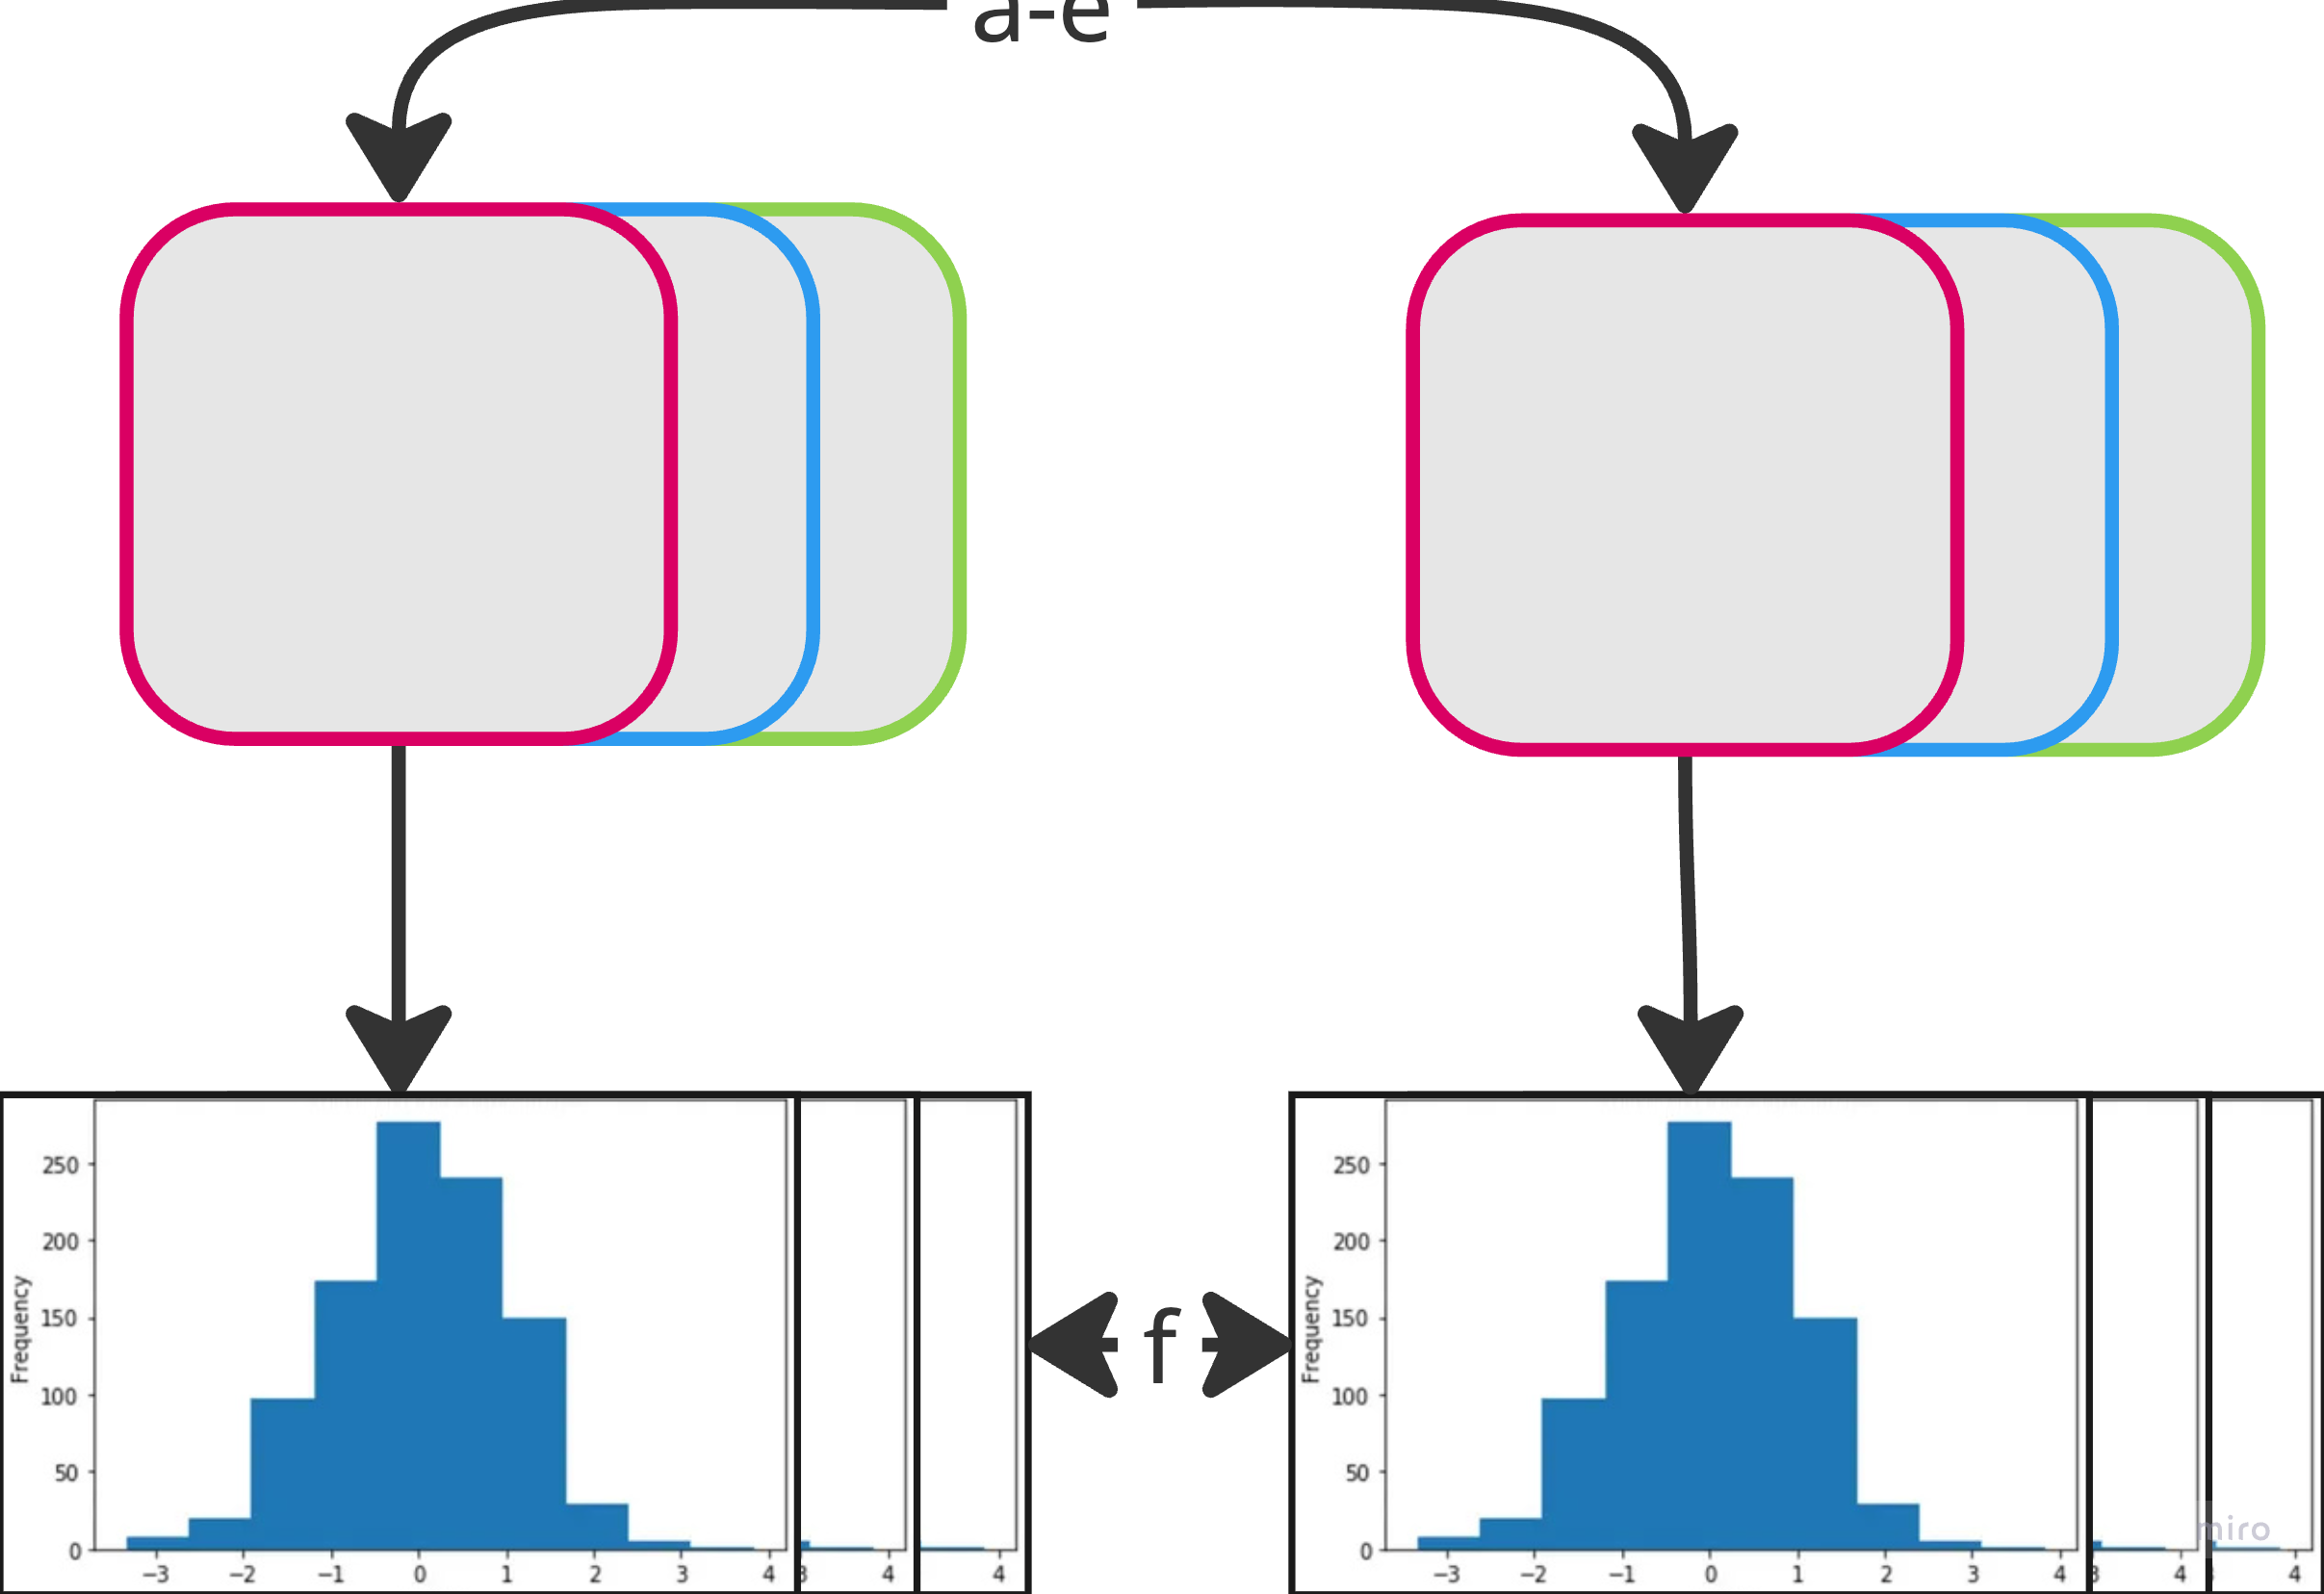
\includegraphics[scale=0.15]{Presentation/Pictures/hist_vectors.png}
    \caption{Векторизация весов модели с помощью гистограмм}
    \label{fg:vectors}
    \end{center}
\end{figure}

Результаты эксперимента представлены в таблице \ref{table:1}. Можно заметить, что автоэнкодеры с линейным слоем, обученные на разных датасетах, отличить друг от друга легче, чем автоэнкодеры со свёрточными слоями. То есть, чем сложнее модель, тем больше информации теряется о ней и датасете при обучении и векторизации.

\begin{table}[!ht]
\begin{center}
\caption{Метрики качества предсказания класса, на котором обучалась модель}
\begin{tabular}{| c | c | c |}
\hline
& Precision & Recall \\ \hline
1 линейный слой & 0.79 & 1.00 \\ \hline
1 свёрточный слой & 0.55 & 0.78 \\ \hline
\end{tabular}
\label{table:1}
\end{center}
\end{table}

\subsection{Предсказане вектора в пространстве датасетов-моделей}

Для базового эксперимента берётся 3 наиболее удалённых класса из датасета CIFAR. Для поиска таких классов использовалось евклидово расстояние на ембеддингах, полученных из выходного слоя ResNet. Архитектура решения представлена на рис \ref{fg:model_2}.

\begin{enumerate}
    \item Случайное сэмплирование долей классов в датасете для $N$ моделей;

    \item Обучение $N$ моделей на соответствующих датасетах;

    \item Получение векторов из обученных моделей;

    \item Обучение энкодера на полученных моделях. Предсказание:
        \begin{enumerate}
            \item Вектора на части единичной сферы

            \item Расстояния между двумя моделями
        \end{enumerate}
\end{enumerate}

\begin{figure}{}
    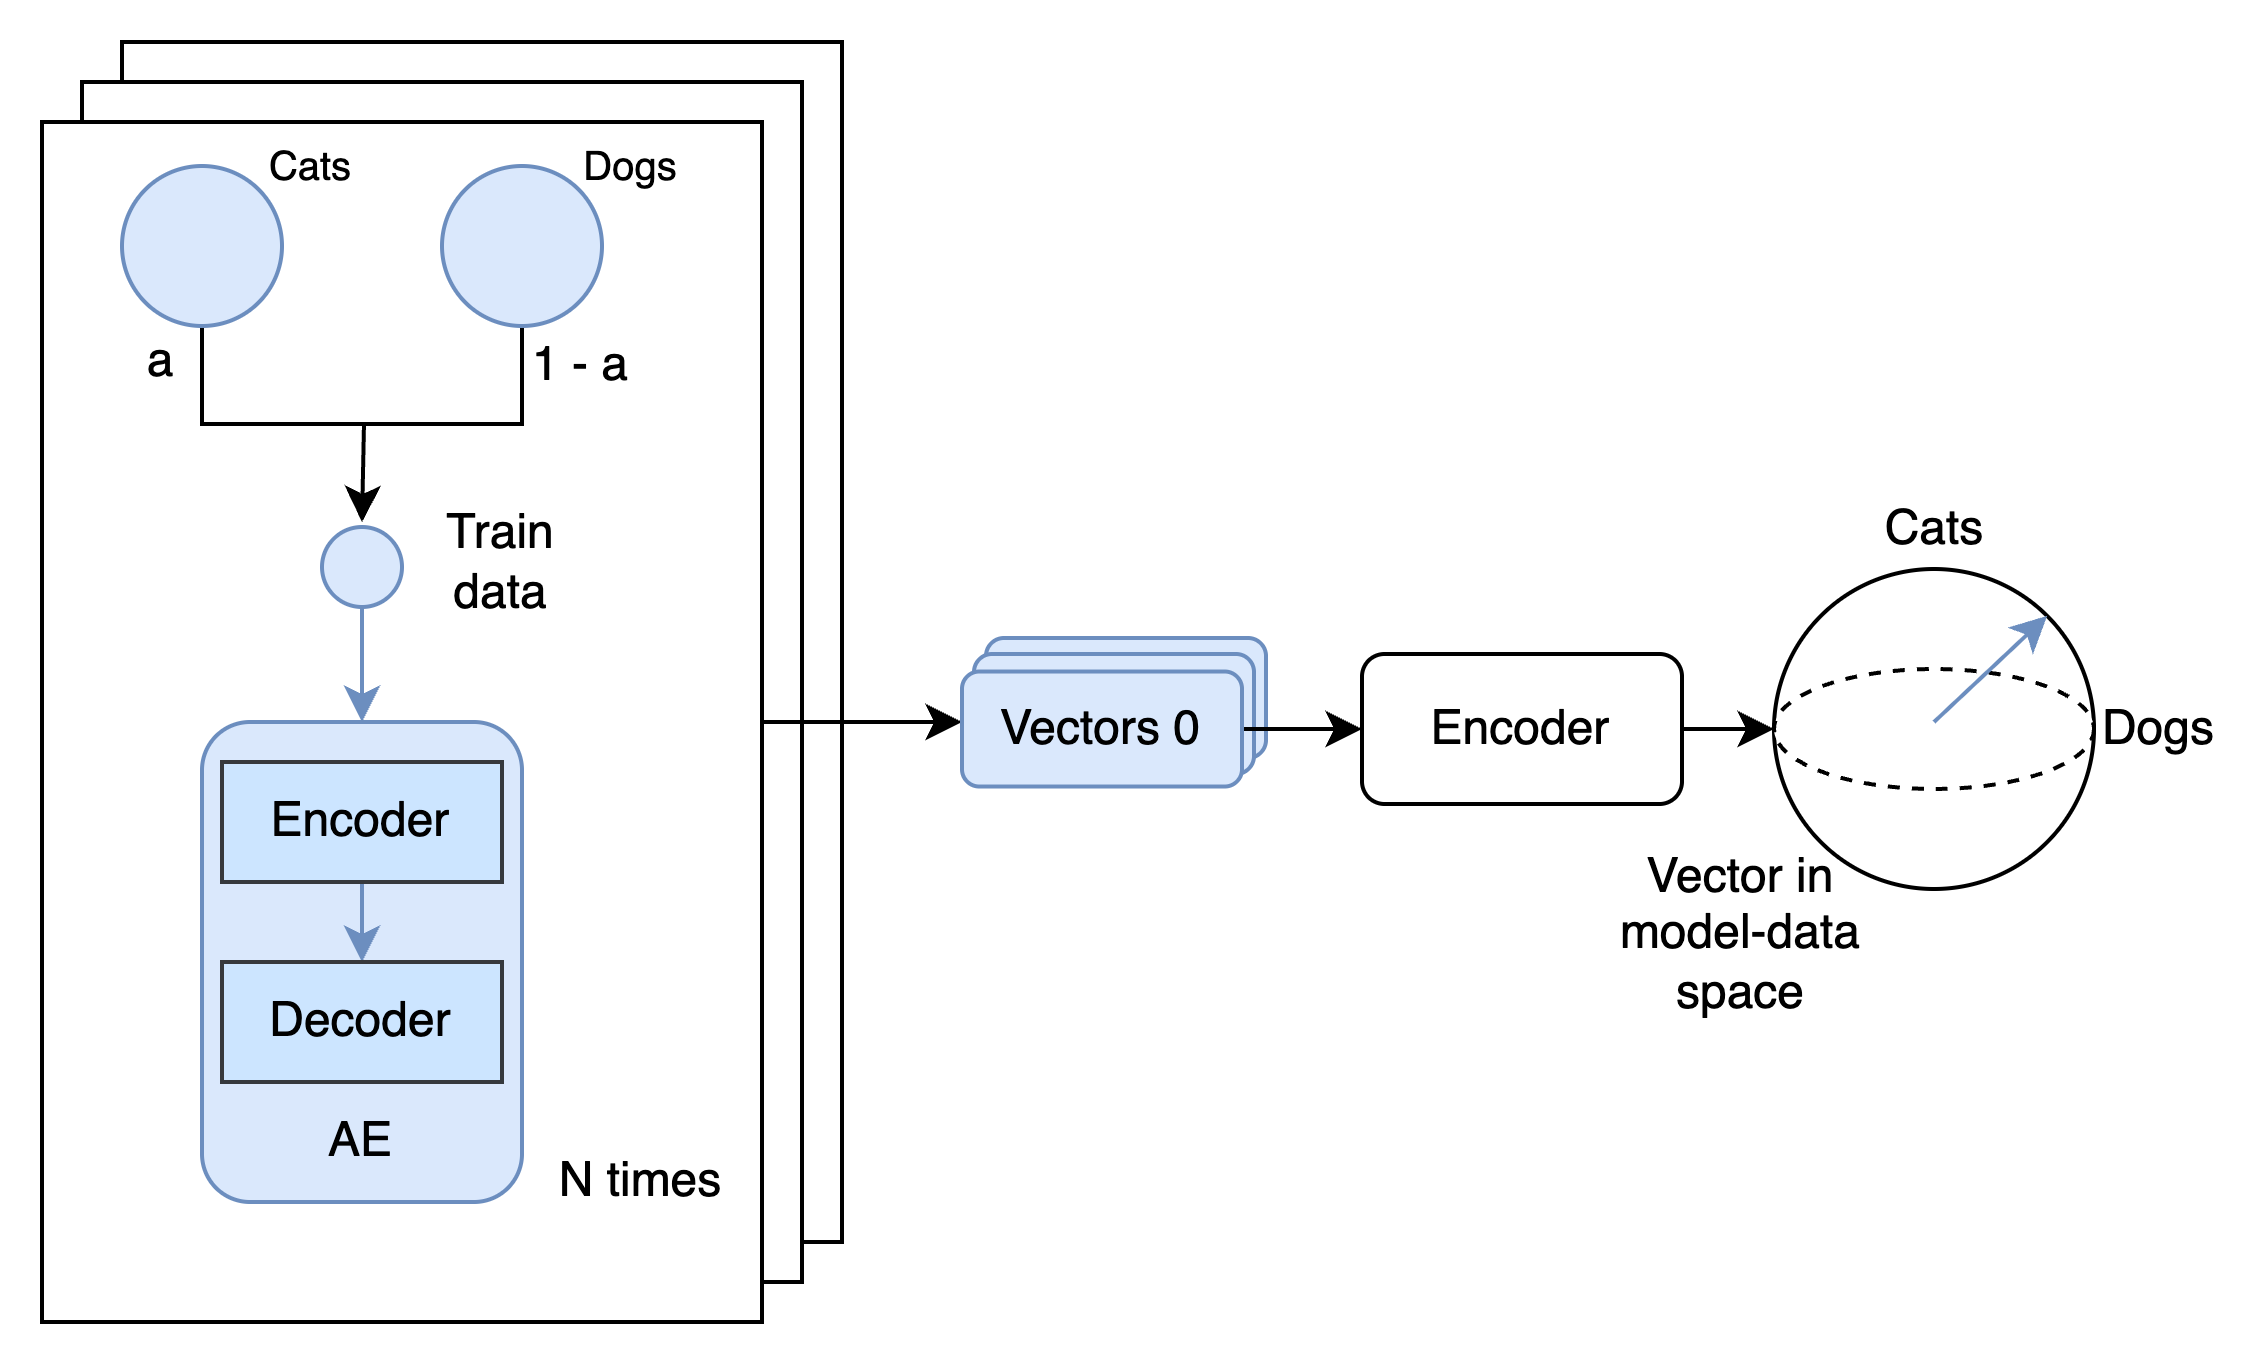
\includegraphics[width=1.0\linewidth]{Presentation/Pictures/experiment.png}
    \caption{Архитектура эксперимента с предсказанием вектора в пространстве датасетов-моделей}
    \label{fg:model_2}
\end{figure}

Функции потерь для реализации обучения:

\begin{enumerate}
    \item Contrastive N-pair loss, где $\text{Encoder}(m_i) = \textbf{x}$, $\textbf{d}_i = \textbf{x}_i^+$, остальные элементы батча: $\textbf{x}_i^-$:

\[\mathcal{L}_{N-pair}(f) = - \log \frac{\exp(\textbf{x}^T \textbf{x}_i^+)}{\exp(\textbf{x}^T \textbf{x}_i^+) + \sum _{i=1}^{N-1} \exp(\textbf{x}^T\textbf{x}_i^-)};\]
    \item Угол между вектором модели $\text{Encoder}(m_i)$ и датасета $\textbf{d}_i$:

\[\mathcal{L}_{cos}(\text{Encoder}(m_i), \textbf{d}_i) = \cos(\text{Encoder}(m_i) \cdot \textbf{d}_i);\]

    \item Triplet loss:

\[\mathcal{L}_{Triplet} = \sum\limits_{x \in \chi}\max(0, ||\textbf{x} - \textbf{x}^+||_2^2 - ||\textbf{x} - \textbf{x}^-||_2^2 + \epsilon;\]

    \item MSE между $\text{Encoder}(m_i)$ и $\textbf{d}_i$:

\[\mathcal{L}_{MSE}(\text{Encoder}(m_i), \textbf{d}_i) = \|\text{Encoder}(m_i) - \textbf{d}_i)\|_2^2.\]
\end{enumerate}

\newpage
\bibliographystyle{plain}
\bibliography{references.bib}
\end{document}